\documentclass[11pt,a4paper]{article}
% Packages every document in this directory shares. Kept apart from
% notation.tex so a symbol change and a package change are separate reviews.
\usepackage[margin=1in]{geometry}
\usepackage{amsmath}
\usepackage{amssymb}
\usepackage{booktabs}
\usepackage{graphicx}
\usepackage{tikz}
\usetikzlibrary{shapes.geometric}
\usepackage{microtype}
\usepackage{algorithm}
\usepackage{algpseudocode}
\usepackage[numbers]{natbib}
\usepackage[hidelinks]{hyperref}

% The one visual vocabulary the problem-statement sketches share. Circles are
% variables, squares are factors, shading marks where an observation enters,
% and a triangle marks a factor that gates on a second variable. Each of the
% eleven sketches carried a private copy, between them four circle diameters,
% three square sizes and four fonts, so a reader learned the convention once
% per figure (issue #529). A figure that needs a shape of its own adds it
% locally, on top of these.
\tikzset{
  fgvariable/.style={circle, draw, fill=white, minimum size=0.58cm,
                     inner sep=0.5pt, font=\footnotesize},
  fgobserved/.style={fgvariable, fill=black!12},
  fgfactor/.style={rectangle, draw, fill=white, minimum size=0.16cm,
                   inner sep=0pt},
  fgdata/.style={fgfactor, fill=black!25},
  fgindicator/.style={fgfactor, fill=black!55},
  fggate/.style={regular polygon, regular polygon sides=3, draw, fill=white,
                 minimum size=0.25cm, inner sep=0pt},
  fglink/.style={draw, thick},
  fgabsent/.style={draw, thin, gray, dashed},
  fgnote/.style={anchor=west, font=\footnotesize}
}

% Shared notation for every document in this directory.
%
% One definition per symbol, input by both the paper and the textbook, so a
% symbol cannot mean two things in two places (issue #249). A document that
% needs a symbol adds it here rather than defining its own; the notation table
% in the textbook is generated from this list by hand and reviewed against it.

% --- Structures ----------------------------------------------------------
\newcommand{\tree}{\mathcal{T}}          % a tree topology
\newcommand{\graph}{\mathcal{G}}         % a general undirected graph
\newcommand{\states}{\mathcal{A}}        % the state alphabet
\newcommand{\rootnode}{\rho}             % the root of a rooted tree
\newcommand{\neighbourhood}{\mathcal{N}} % a discrete move neighbourhood

% --- Continuous parameters ------------------------------------------------
\newcommand{\Q}{\mathbf{Q}}              % a rate matrix
\newcommand{\Pmat}{\mathbf{P}}           % a transition probability matrix
\newcommand{\SubMat}{\mathbf{S}}         % a symmetric exchangeability matrix
\newcommand{\bpi}{\boldsymbol{\pi}}      % a stationary or initial distribution
\newcommand{\branch}{\boldsymbol{\tau}}  % branch lengths
\newcommand{\params}{\boldsymbol{\theta}}% unconstrained parameters
\newcommand{\constrained}{\phi}          % the constraint map

% --- Data and objectives --------------------------------------------------
\newcommand{\data}{\mathbf{D}}           % observed data
\newcommand{\objective}{\mathcal{L}}     % the scalar being optimized
\newcommand{\energy}{H}                  % a Hamiltonian
\newcommand{\hidden}{\mathbf{Z}}         % a hidden state path
\newcommand{\emission}{\mathcal{E}}      % an emission family

% --- Reading a generated caption -----------------------------------------
% The captions under figures/ are written by the QA build, never by hand
% (docs/CLAUDE.md). This reads one in so a document quotes it rather than
% restating it.
\newread\qacaptionfile
\newcommand{\qacaptionread}[2]{%
  \begingroup
  \endlinechar=-1
  \openin\qacaptionfile=#1\relax
  \global\read\qacaptionfile to #2
  \closein\qacaptionfile
  \endgroup
}


\title{Mixed Discrete-Continuous Optimization for Graph-Structured Models: \\
Applications in Phylogenetics, Potts Models, and Hidden Markov Models}
\author{M.\ J.\ Wilson}
\date{\today}

\begin{document}
\maketitle

\begin{abstract}
\noindent
Inference over graph-structured models---phylogenetic trees, lattice-based
Potts models, hidden Markov models, and the low-density parity-check codes
that share their message passing---is a coupled discrete-continuous
optimization problem. The structural search space is combinatorial, while
scoring each candidate structure requires continuously optimizing its
parameters. We present a framework that strictly decouples differentiable
continuous optimization from discrete structural search, so that one optimizer
serves every model class and a structural move constructs a new objective
rather than taking a step inside an existing one. Framing structural search
as a Markov decision process admits learned proposal policies, a critic and
a planner over exact, approximate, bounded or learned surrogate objectives.
We validate the engine against exact oracles---brute-force marginalization,
path enumeration, and exhaustive topology enumeration---and report realized
interval coverage rather than asserting it. Every comparison between methods
is run at an equal budget of objective evaluations over shared seeds with a
paired test, and the negative results are reported beside the positive ones:
restarts are not beaten on the continuous surfaces measured, a learned tree
policy ties hill climbing on the one fixture that separates them, and no
site reaches a two-fold speedup from process parallelism on a four-core host.
Formulations, algorithms, and the properties each is validated against are
given in the companion textbook; this paper reports results.
\end{abstract}

\tableofcontents

\section{Introduction}
\label{sec:intro}

The fundamental difficulty in high-dimensional probabilistic inference is the
combinatorial size of the structural search space. In phylogenetics, the number
of unrooted binary topologies over $n$ taxa is $(2n-5)!!$ \citep{rosen2019}. In
statistical physics, the ground state of an $N$-dimensional Potts model
requires traversing an exponentially large configuration space
\citep{mezard2009}. Decoding a hidden Markov model poses the same coupled
problem on a chain \citep{mackay2003}, and decoding a low-density parity-check
code poses it on the sparse bipartite graph of a code's parity checks, where
the sum-product algorithm was rediscovered as belief propagation
\citep{kschischang2001}. The four are one marginalization over four
structures, and two derived instances sit between them: a coupled
spatio-sequential model, a Potts prior over class labels gating one hidden
chain per class, and the Gaussian mixture, a hidden Markov model with the
chain removed.

Classical frameworks rely on fixed, hand-designed heuristics---nearest-neighbour
interchange for trees, Swendsen--Wang cluster updates for lattices---applied
greedily or under simulated annealing. This paper builds those baselines
first, pins each to an oracle, and only then asks whether a learned component
beats them: a policy over the same neighbourhoods trained by the
score-function estimator, an actor--critic and proximal policy optimization,
a planner with the policy as prior and the critic as leaf value, certified
bounds and learned surrogates that rank a neighbourhood before it is fitted,
and a continuous relaxation of the discrete configurations. The continuous
parameters are fitted by reverse-mode automatic differentiation throughout.

\subsection{Scope}
This paper reports what has been built and measured. The formulations it
rests on---the substitution model, the Potts energy, the hidden Markov
recursions, the discrete move sets, the decision process, the bounds, and the
mathematical properties each algorithm is refereed by---are stated in the
companion textbook rather than repeated here. Three things are outside it and
are stated as such rather than left implicit. The low-density parity-check
class has its simulator, decoder and oracles and no move set yet, so it
appears in Section~\ref{sec:res-likelihood} and not in the search results.
No comparison against IQ-TREE~2 or RAxML-NG has been run: no external solver
is admitted, and adopting one is a deferred decision of its own (\#126). And
no accelerator exists to measure on, so hardware scaling is reported for the
CPU alone.

\section{Methods}
\label{sec:methods}

The methodology rests on one division: continuous parameters are optimized by
gradients on a fixed structure, while discrete structural moves are proposed by
an external agent and construct an entirely new differentiable objective. A
move changes what the parameter vector means and how long it is, so it cannot
be a step inside a fit over a fixed-length vector.

\subsection{Continuous optimization}
An objective is a differentiable scalar $\objective(\params)$ over an
unconstrained vector $\params \in \mathbb{R}^d$, with an injective map
$\constrained$ to the constrained parameters the model is stated in. The same
quasi-Newton optimizer \citep{nocedal2006} therefore minimizes negative
log-likelihoods of phylogenetic alignments, free energies of Potts models,
sequence log-likelihoods of hidden Markov models, the mixture likelihood and
three closed-form test functions without knowing which it has. Standard errors
come from the observed information at the optimum, pushed through
$\constrained$ by the delta method, at any fit whatever produced it---an
expectation--maximization fit inverts the same constraint map to be given the
same interval---and are refused where the information is singular. A
Hamiltonian sampler over the same interface gives an interval as a posterior
quantile instead, with a warm-up that adapts its step and mass matrix and a
parallel-tempering ladder chosen from its measured exchange acceptance.

\subsection{Differentiable likelihoods and energies}
Partial likelihoods are evaluated by a post-order recursion, with branch
lengths $\branch$ and the rate matrix $\Q$ kept inside the automatic
differentiation graph, so gradients are exact rather than numerical
\citep{goodfellow2016, prince2023}. Rescaling against underflow is part of that
graph. The Potts energy is normalized by a transfer matrix on a chain and by
belief propagation on a lattice; the hidden Markov evidence by the forward
recursion, with forward--backward exposed as an evaluator; and all of them by
one sum-product and max-product implementation over a factor graph that also
expresses the coupled model, pinned to each specialized evaluator and slower
than it, so the specialized evaluators stay.

\subsection{Discrete search and its surrogates}
Hill climbing over nearest-neighbour interchange or subtree
prune-and-regraft fits the continuous parameters of every candidate, counts
its budget in candidates scored, and scores each topology once. A neighbour
starts its fit from its parent's branch lengths matched by leaf split, and a
neighbourhood may be ranked by one cached evaluation, by a certified analytic
bound, or by a learned predictor before only the top candidates are fitted;
the accepted move is always fitted in full. Large parsimony runs the same
climb on the Fitch or Sankoff score. Potts ground states are exact by minimum
cut where the couplings are submodular, within a proved factor by alpha
expansion above two states, and bounded by a semidefinite relaxation where
the couplings are negative; samplers, annealing and parallel tempering run
over one temperature schedule, and a Gibbs sampler and annealer over any
factor graph.

\subsection{Structural search as a Markov decision process}
\label{sec:rl}
Discrete graph traversal is formulated as a Markov decision process
\citep{suttonbarto2018}: the \textbf{state} is the current structure, its
optimized continuous parameters, and observation summaries; an \textbf{action}
is a structural perturbation from a classical neighbourhood; the
\textbf{reward} is the improvement in the objective. Every learning claim is
pinned to an oracle before it is measured: on an environment small enough to
enumerate, the expected return, its gradient, the action values and the
optimal value are exact. On that footing the score-function estimator with a
baseline, an actor--critic with a fitted critic, proximal policy optimization
with generalized advantage estimation and an optional epsilon-greedy
behaviour policy, and a planner running PUCT search with the policy as prior
and the critic as leaf value, trained by expert iteration, are compared at
matched budgets. A Gumbel-softmax relaxation of Potts configurations and
hidden state paths is the differentiable alternative, admitted where its
optimum is enumerable so the claim is falsifiable.

\subsection{Budgets and the ledger}
Every comparison between methods spends an equal budget in one declared
unit---candidate fits, sweeps, or objective evaluations---over shared seeds,
derives the restart baseline's count from that budget, refuses a method that
spends past it, and reports an exact McNemar test on the paired hits. The
measured comparisons are recorded in an experiment ledger, one file per
experiment against its commit, and cited here by number.

\section{Results}
\label{sec:results}

Every figure below is rendered from the code it reports on and carries a
generated caption naming the seed, sizes, and model that produced it.

\subsection{Simulation against its analytic truth}
\label{sec:res-simulation}

\qacaptionread{figures/sim_example_caption.txt}{\simExampleCaption}
\begin{figure}[htbp]
  \centering
  \includegraphics[width=0.8\linewidth]{figures/sim_example}
  \caption{\simExampleCaption}
  \label{fig:sim-example}
\end{figure}

\subsection{Exact inference across backends}
\label{sec:res-likelihood}

The pruning backends are held to brute-force marginalization
(Figure~\ref{fig:backend-agreement}). The other evaluators are held the same
way, and the parity-check decoder is the newest: on a cycle-free 22-bit code
its posteriors equal the tree-schedule sum-product and the enumeration over
all 32,768 codewords to $1.9 \times 10^{-13}$ in log-odds, min-sum returns the
enumerated maximum-likelihood codeword, and on six loopy codes it reaches the
general damped flooding's fixed point within $4.6 \times 10^{-11}$. At 19,998
bits, where no enumeration reaches, the (3,6) code resolves every erasure at
an erasure probability of 0.42 on three seeds and leaves 25 to 30\% of its
bits erased at 0.44, bracketing the density-evolution threshold 0.4294.

The turbo code is the second member of that class, and it separates two
things the parity-check code does not. One constituent convolutional code is
a terminated trellis, so it is a chain and BCJR on it is exact: its bit
posteriors equal the sum over all $2^{K}$ messages to $2.8 \times 10^{-14}$
in log-odds, and the tree schedule of the general sum-product on the same
chain, built as a factor graph, agrees to $2.7 \times 10^{-15}$ with the same
$\log Z$. The pair is not: two chains sharing the message bits through an
interleaver have cycles, and the iteration between them is the Bethe
approximation. What is reported there is the gap rather than an equality. At
$K = 12$, where enumeration reaches, eight iterations give a bit error rate
1.26 to 3.20 times the exact bitwise MAP's over four operating points and
1,200 message bits each; the code is worse than sending the bits uncoded at
$0$~dB, which is a property of a 12-bit interleaver and not of the decoder.
At $K = 1{,}024$ over 200 frames per point the curve falls two orders of
magnitude between $0$ and $1.2$~dB and stays below the uncoded
$Q(\sqrt{2E_b/N_0})$ throughout (Figure~\ref{fig:turbo-waterfall} in the
textbook draws the $K = 256$ instance). Two negative results travel with it.
The ensemble bit error rate is not monotone in the iteration count: it rises
between consecutive iterations at four of six operating points, the largest
rise $2.3 \times 10^{-3}$, and every rise is inside one binomial interval of
the sample, so the strong claim is refused and the weak one---no worse, and
better than the first iteration---is what the suite asserts. And a bit error
rate is reported with the frame count behind it in every case, because a
waterfall without one bounds nothing.

Collapsing identical alignment columns to weighted site patterns leaves the
log-likelihood unchanged and cuts the column work by 1.6 to 781 times across
the fixtures, the ratio set by the taxon count against the site count rather
than by either alone. It saturates at $k^{\,n}$ distinct columns, so the same
trick over blocks of $N > 1$ consecutive sites buys a bracket instead: the
blocks occurring at least $m$ times are evaluated exactly and the rare tail is
bounded by the extremes of a single site's log-likelihood, had in one pass
over the tree. The bracket contains the exact value on every fixture and on
uniform-random alignments, over block sizes 1 to 5 and cutoffs 1 to 32, and
its width is exactly the bounded site count times the per-site range: at five
taxa and 2,000 sites, $1.0\,|\ell|$ at $N = 1$ and $m = 8$, and $2.8\,|\ell|$
once $N \ge 3$ leaves the whole alignment in the tail. Neither end therefore
orders topologies; the frequent blocks' own log-likelihood does, and ranking
by it reaches the same optimum as fitting every candidate at 2 to 4 fits
against 5 to 15.

\qacaptionread{figures/backend_agreement_caption.txt}{\backendAgreementCaption}
\begin{figure}[htbp]
  \centering
  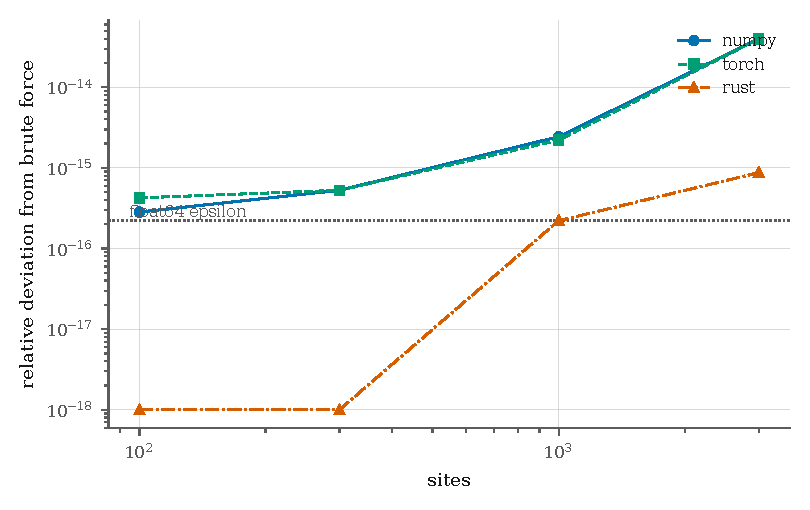
\includegraphics[width=0.8\linewidth]{figures/backend_agreement}
  \caption{\backendAgreementCaption}
  \label{fig:backend-agreement}
\end{figure}

\subsection{Parameter recovery and interval coverage}
\label{sec:res-recovery}

Recovery is the acceptance test for a fit, and a Wald interval from the
observed information is an \emph{asymptotic} claim. The figures below are
the evidence for it rather than an assertion of it: the first shows each fitted
parameter of the Potts chain and the hidden Markov model against the value
that generated the data, the second the realized coverage against the amount
of data each fit sees, and the third and fourth the phylogenetic instance,
branch lengths and the general time-reversible model, where two directions
of the parameter space are gauges and are fitted as such.

\qacaptionread{figures/opt_recovery_caption.txt}{\optRecoveryCaption}
\begin{figure}[htbp]
  \centering
  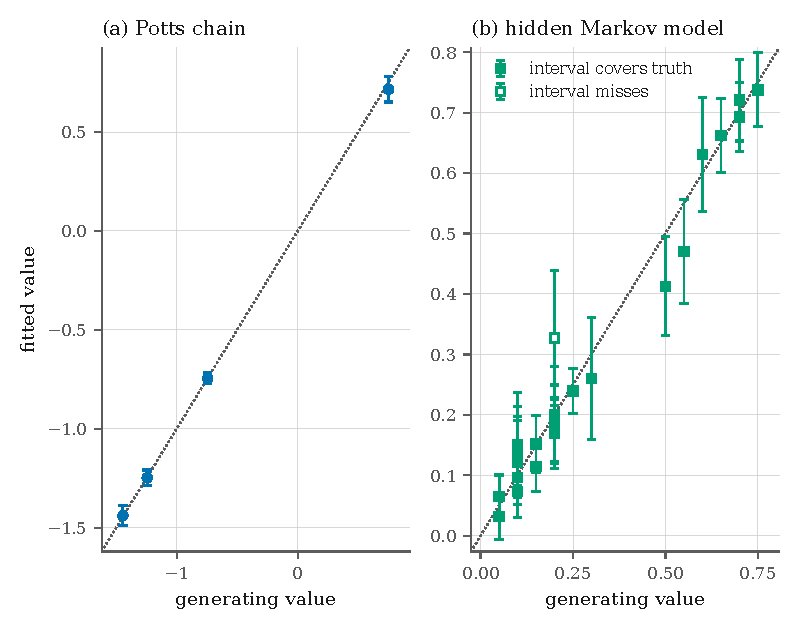
\includegraphics[width=0.9\linewidth]{figures/opt_recovery}
  \caption{\optRecoveryCaption}
  \label{fig:opt-recovery}
\end{figure}

\qacaptionread{figures/opt_coverage_caption.txt}{\optCoverageCaption}
\begin{figure}[htbp]
  \centering
  \includegraphics[width=0.75\linewidth]{figures/opt_coverage}
  \caption{\optCoverageCaption}
  \label{fig:opt-coverage}
\end{figure}

\qacaptionread{figures/opt_branch_recovery_caption.txt}{\optBranchRecoveryCaption}
\begin{figure}[htbp]
  \centering
  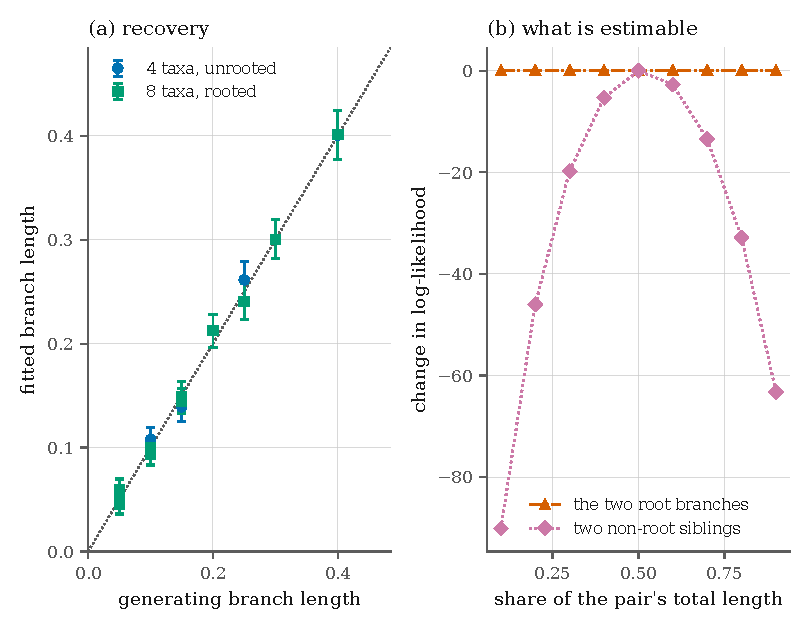
\includegraphics[width=0.9\linewidth]{figures/opt_branch_recovery}
  \caption{\optBranchRecoveryCaption}
  \label{fig:opt-branch-recovery}
\end{figure}

\qacaptionread{figures/opt_model_recovery_caption.txt}{\optModelRecoveryCaption}
\begin{figure}[htbp]
  \centering
  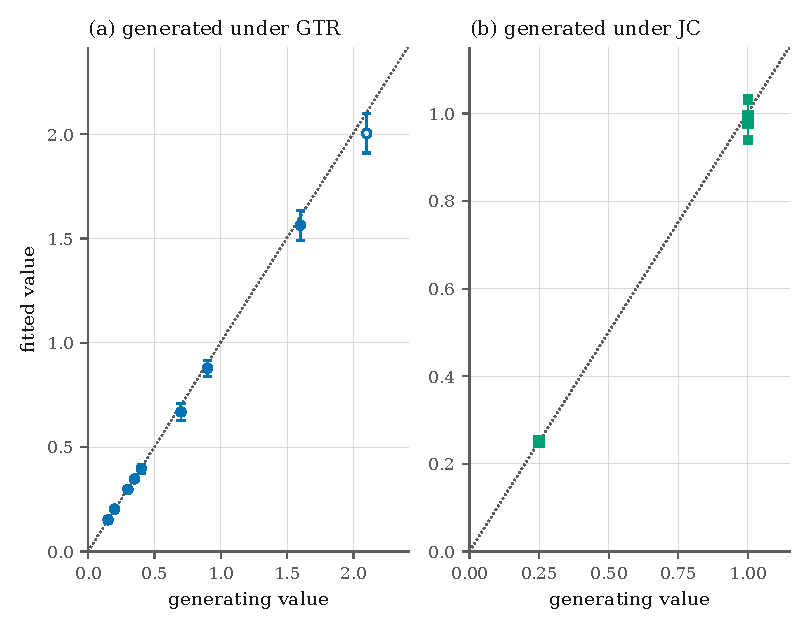
\includegraphics[width=0.9\linewidth]{figures/opt_model_recovery}
  \caption{\optModelRecoveryCaption}
  \label{fig:opt-model-recovery}
\end{figure}

\subsection{Discrete search against exhaustive enumeration}
\label{sec:res-search}

Below the size at which every topology can be enumerated, enumeration is the
only independent statement available about whether a search found the best tree
or merely a good one. The first figure is the climb and the landscape it
climbed; the second the tree it selected beside the best one it rejected.

\qacaptionread{figures/search_trajectory_caption.txt}{\searchTrajectoryCaption}
\begin{figure}[htbp]
  \centering
  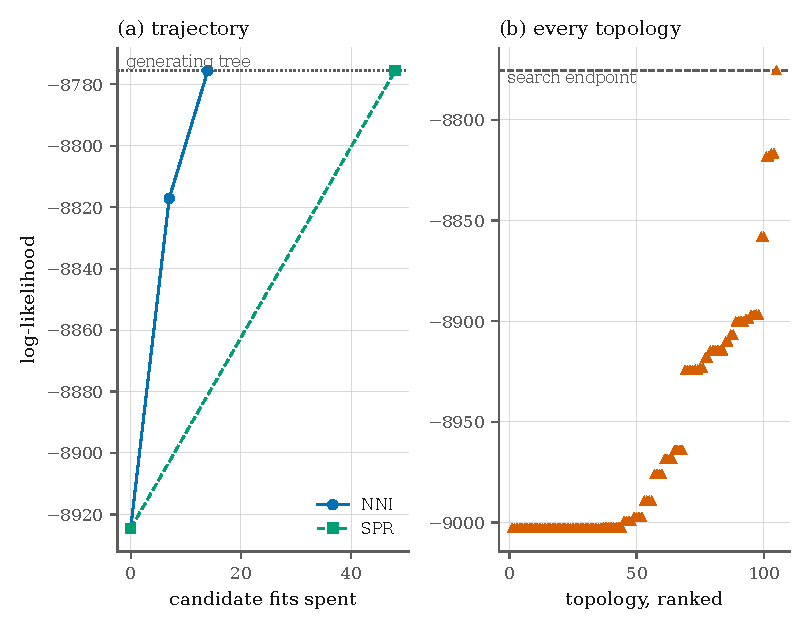
\includegraphics[width=0.8\linewidth]{figures/search_trajectory}
  \caption{\searchTrajectoryCaption}
  \label{fig:search-trajectory}
\end{figure}

\qacaptionread{figures/search_topologies_caption.txt}{\searchTopologiesCaption}
\begin{figure}[htbp]
  \centering
  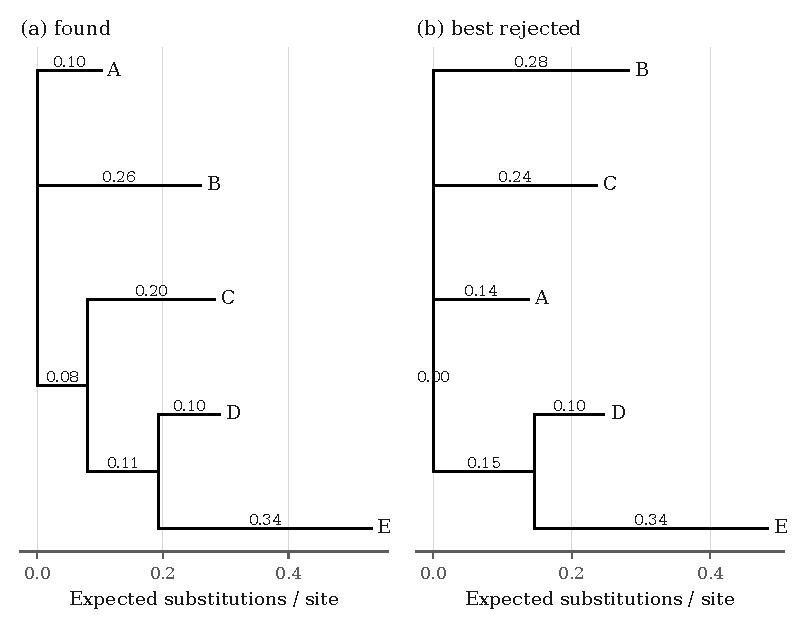
\includegraphics[width=0.8\linewidth]{figures/search_topologies}
  \caption{\searchTopologiesCaption}
  \label{fig:search-topologies}
\end{figure}

\subsection{Differentiable topology search}
\label{sec:res-tropical}

The space of trees on $n$ leaves is the tropical Grassmannian
$\mathrm{Gr}(2,n)$ \citep{speyer2004}, a quartet's resolution is the
$\arg\min$ of three linear forms in its coordinates, and softening that
$\arg\min$ makes the topology differentiable
(the companion textbook states the construction). What the roadmap
recorded as missing was the referee, and enumeration supplies one below nine
taxa.

At the tree metric of every one of the 15, 105 and 945 topologies of the
five-, six- and seven-taxon fixtures, and of 201 of the 10{,}395 at eight, the
relaxation equals the discrete quartet score to $3.8\times10^{-16}$ of its
magnitude, at a temperature derived per corner from that corner's own quartet
gaps rather than chosen. The softmin's own contribution is certified under
$10^{-11}$; what is left at that temperature is float64 rounding of a sum over
$\binom{n}{4}$ terms, which is why the agreement is pinned relatively.
The relaxation's $\arg\min$ reading of a quartet agrees with the tree's leaf
bipartitions over all 1{,}065 topologies at the first three sizes. The
Hadamard conjugation of the exact two-state spectrum returns a metric whose
four-point violation is below $10^{-12}$ and which resolves every quartet as
the generating tree does --- a point of $\mathrm{Gr}(2,n)$ from a closed form
sharing no algebra with a walk over the tree.

\qacaptionread{figures/tropical_relaxation_caption.txt}{\tropicalRelaxationCaption}
\begin{figure}[htbp]
  \centering
  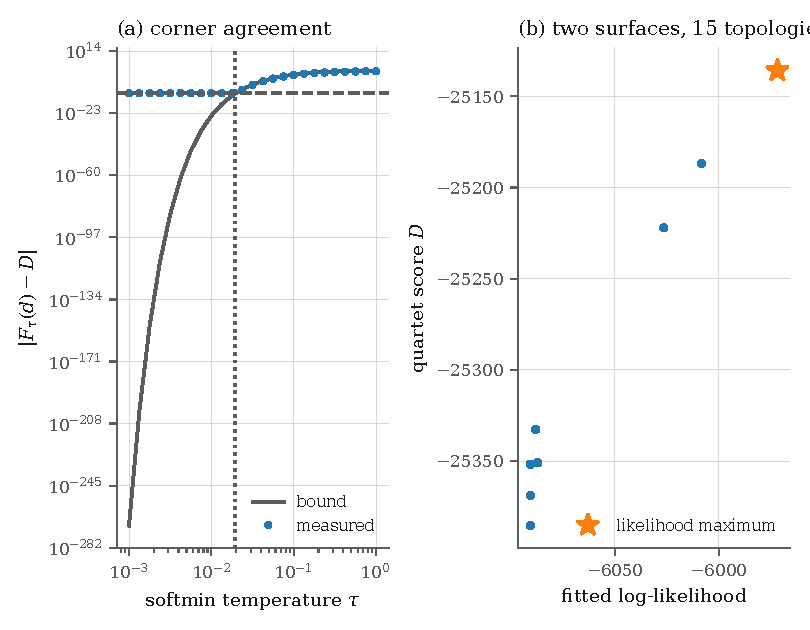
\includegraphics[width=0.8\linewidth]{figures/tropical_relaxation}
  \caption{\tropicalRelaxationCaption}
  \label{fig:tropical-relaxation}
\end{figure}

What the relaxation buys is a separate question and on these fixtures the
answer is nothing. Annealed ascent from 8 random metrics reaches the
enumerated maximum of the quartet surface 8 of 8 times at five and six taxa
and 7 of 8 at eight, the miss stopping at the runner-up, $15.8$ below in
$302{,}287$. Neighbor joining on the estimated distances reaches the same
maximum on every fixture measured, at no gradient steps. The quartet surface
shares its maximizer with the fitted likelihood at five and six taxa, where
both enumerate. On the seven-taxon fixture chosen so that hill climbing fails,
the top two quartet scores differ by $0.0117$ in $339{,}982$ ---
$3.4\times10^{-8}$, inside the convergence of the fits that produced them ---
so the enumerated maximum is not a target any method can be held to there, and
both the relaxation and neighbor joining return the generating topology.
Ascent leaves the variety: the four-point violation where it stops is $0.24$,
$0.05$, $2.15$ and $1.04$ in units where the metric has mean 1, and at seven
taxa its relaxed value exceeds every corner's by $0.96$, which is the outer
relaxation's gap measured rather than assumed absent. No budget-matched claim
is made against the bounded-radius search of Section~\ref{sec:res-budget}:
the relaxation costs $3\binom{n}{4}$ four-taxon fits, 15 to 210 over these
sizes, against that search's 31 six-taxon fits, and no fixture measured here
separates the two on quality.

\subsection{The reward an agent can afford}
\label{sec:res-reward}

Fitting branch lengths per candidate costs a full optimization where scoring
at fixed parameters costs one pruning pass, and only the second makes an
episode affordable. The substitution is validated rather than assumed: the
two surfaces agree on the best topology and correlate at 0.9568 on the
six-taxon fixture, and the agreement holds across a 50-fold range of the
fixed branch length.

\qacaptionread{figures/rl_reward_surface_caption.txt}{\rlRewardSurfaceCaption}
\begin{figure}[htbp]
  \centering
  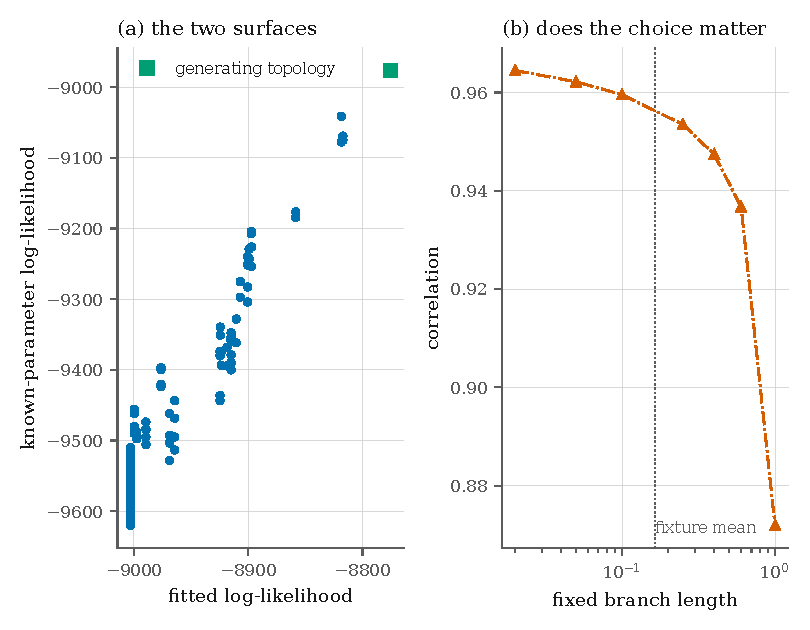
\includegraphics[width=0.8\linewidth]{figures/rl_reward_surface}
  \caption{\rlRewardSurfaceCaption}
  \label{fig:rl-reward-surface}
\end{figure}

\subsection{Learned proposals against hill climbing}
\label{sec:res-learning}

Where the landscape can be enumerated, learning is refereed by the exact
expected return. On the Potts chain the reward decomposes into the two
features the policy scores, which puts hill climbing inside the policy class:
the learned policy reaches the enumerated optimum from 86.6\% of the 81 starts
against greedy's 80.2\%, in 8 of 8 training seeds (ledger entry 003); at the
same budget the actor--critic reaches it from 88.9\% and proximal policy
optimization from 96.3\%, and at a quarter of the budget 87.7\% against the
score-function estimator's 32.1\%. A planner with a trained prior and critic
reaches it from 92.6\% of starts at 8.3 successor evaluations per episode
against greedy's 80.2\% at 48, and matches greedy at 6.3.

Figure~\ref{fig:rl-convergence} poses the phylogenetic comparison on a
topology landscape where hill climbing demonstrably fails, which is the
condition that makes the comparison askable at all: on a landscape the
baseline already solves from every start, a policy can be neither better nor
worse than it. The answer is a tie. Every algorithm---the score-function
estimator, the actor--critic, proximal policy optimization on and off
policy---lands on greedy's 0.48 within the 0.014 standard deviation over
seeds, because the environment exposes one feature, the improvement a move
buys, so the policy is an inverse temperature and no algorithm can learn
what that class cannot express. Random-restart hill climbing reaches the
enumerated maximum from every start at the same 60-decision budget, so the
baseline the next comparison has to beat is 1.000 and a fixture that
separates anything from restarts is what it needs. Given something to learn
the policy learns: with seven columns per move---the improvement, the
parsimony change, the pattern support of the split broken and of the split
made, and the two exchanged subtree sizes---it reaches the maximum from
0.796 of episodes at the same budget, ahead of greedy on 16 of 16 seeds
($p = 3.05 \times 10^{-5}$, ledger entry 005), and is not yet measured
against restarts.

\qacaptionread{figures/rl_tree_policy_caption.txt}{\rlTreePolicyCaption}
\begin{figure}[htbp]
  \centering
  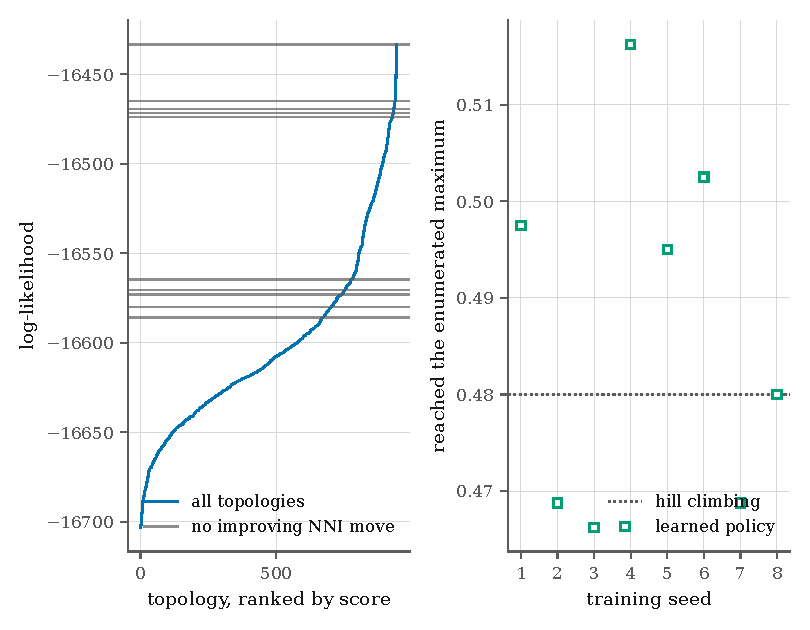
\includegraphics[width=0.8\linewidth]{figures/rl_tree_policy}
  \caption{\rlTreePolicyCaption}
  \label{fig:rl-convergence}
\end{figure}

\subsection{Budgeted comparisons}
\label{sec:res-budget}

Which search wins is a property of the instance, and every comparison below
is at an equal budget over shared seeds. On the planted Viana--Bray spin
glass at 60 sites, degree 4 and frustration 0.2, at 400 sweeps per method
over 12 instances, parallel tempering reaches the best energy any method
found on 12 of 12, annealing on 10 of 12 with a mean gap of 0.17, and
restarts of descent on 4 of 12 with a mean gap of 0.75; every method beats
the planted energy. On the five-component Gaussian mixture at 3,000
likelihood evaluations per start over 40 shared starts, restarts of
expectation--maximization reach the best-known optimum from 7 starts,
parallel tempering from 4 ($p = 0.549$ against restarts) and annealing from
1 ($p = 0.031$), with mean gaps of 2.6, 4.2 and 8.0 nats (ledger entry 004).
On Rastrigin, held to eight fits, neither multi-start nor annealing reaches
the global minimum from any of 10 starts. Three economies of the topology
climb are compared the same way, at a budget of 500 candidates over 8 seeds
and refereed by enumeration: a parsimony start, a regraft bounded to radius
$r$, and refitting only the branches a move changed each reach the enumerated
maximum from every start at five and six taxa, at 1,902, 755 and 1,810 forward
passes against the unbounded search's 2,848 at six taxa, and together at
1,009. At eight taxa, past enumeration, all three together return the
unbounded search's log-likelihood for 1,930 and 3,359 passes against 16,600
and 24,493. Restarts are therefore not beaten
on the continuous surfaces measured and are beaten on the frustrated
lattice, the one instance class past enumeration the roadmap needs. On an
antiferromagnetic chain whose optimum needs coordinated flips the
deterministic relaxation reaches it from 18 of 40 seeds against greedy's 5
($p = 0.00098$), and every sampled variant of it ties at 11 ($p = 0.18$).
At the Potts critical coupling, single-site sampling slows by 3.2 times
between lattice extents 8 and 24 while the cluster moves slow by 1.9
(ledger entry 001). The comparison against classical phylogenetic software
is ticketed (\#126) and not run.

\subsection{Hardware scaling}
\label{sec:res-hardware}

No accelerator exists in the environment, so what is measured is the CPU.
The Rust pruning backend runs at 2.5 times the NumPy oracle at 200 taxa by
11,000 sites, with peak memory 22.6\,MB, and the minimum-cut kernel at 26 to
32 times the reference as a kernel and 6.3 to 10.7 times as a caller sees it,
the difference being the Python energy evaluation and not the boundary copy.
Laying the pruning kernel's partial likelihoods out with sites contiguous and
walking them in tiles, so its inner loops are contiguous, unaliased and free of
early exits, cuts the kernel by 28\% at four taxa by 200,000 sites and 35\% at
eight; through the binding at 11,000 sites it changes nothing measurable, the
call there being 199 internal nodes and a logarithm per site per node rather
than the message pass. The layout was chosen by benchmark and no vector width
is asserted anywhere.
Process parallelism over independent tasks---the multi-start fit, the
budgeted comparison, the bootstrap---was measured on a four-core host at 1, 2
and 4 workers with the intra-op thread count at 1 and at the default: no
site reaches a two-fold speedup at 4 workers, the pool's spawn and import
costing 1.81\,s, more than the multi-start fit does in total, while the
serial fit at the default thread count runs 2.87 times the fit at one thread
because the tensor library already parallelizes over sites. All three sites
stay serial by recommendation, with the argument kept for a larger tier or
machine. Table~\ref{tab:likelihood-footprint} settles the memory
requirement: the roadmap bounds the working set to $O(n \times L \times k)$
inside 16\,GB, the simulator retains every node's states and pruning retains
a partial likelihood only for nodes whose parent has not yet consumed it,
and both are reported on a caterpillar, the deepest tree on its leaves, so
the bound is tight rather than loose.

\qacaptionread{figures/likelihood_footprint_caption.txt}{\likelihoodFootprintCaption}
\begin{table}[htbp]
  \centering
  \begin{tabular}{rrrrr}
  \toprule
  Taxa & Sites & Simulate (MB) & Evaluate (MB) & Total (MB) \\
  \midrule
  20 & 2000 & 0.624 & 2.43 & 3.06 \\
  20 & 11\_000 & 3.43 & 13.4 & 16.8 \\
  100 & 11\_000 & 17.5 & 69.7 & 87.2 \\
  \midrule
  1000 & 11\_000 & 176 & 703 & 879 \\
  \bottomrule
\end{tabular}

  \caption{\likelihoodFootprintCaption}
  \label{tab:likelihood-footprint}
\end{table}

\section{Discussion}
\label{sec:discussion}

Three findings recur across the problem classes, and each is a statement
about the instance rather than about the algorithms. First, most fixtures are
too easy to separate methods: the six-taxon tree is solved from every start,
the Potts chain's optimum is a constant, the triangular antiferromagnet is
reached by restarts of descent as often as by annealing, and it took a
planted glass past enumeration and a seven-taxon tree with short internal
branches to make a comparison askable. The budgeted comparison is therefore
run before any claim is made, and a fixture that fails to separate methods
is recorded as such. Second, where a learned component loses or ties, the
cause is named and measured rather than argued: the tree policy ties greedy
because its feature set is one number, and the relaxation's sampled variants
tie greedy because the sampling, not the relaxation, is what costs. Third,
the negative engineering results are as load-bearing as the positive ones:
the fourth-order integrator loses to leapfrog at equal gradient evaluations,
k-means++ seeding buys nothing the likelihood can use, warm starts save less
than lazy scoring, and process parallelism buys nothing at the mid-size tier.
Each stays as a measured decision rather than a default that moved.

What referees each method is read from the suite and typeset in the
companion textbook: where an oracle is affordable at a size the method is
pinned to it, and where none is, recovery of the simulated truth stands in
while the oracle remains desired. The cells where that second case holds are
marked there, and the oracle each would need is named---a certified
branch-and-bound bound for trees past the enumerable taxon count, a
boundary contraction for lattices past the transfer-matrix width, and
density evolution for codes past the enumerable length.

\section{Conclusions}
\label{sec:conclusions}

Decoupling structural exploration from continuous fitting yields a
model-agnostic optimization engine that serves phylogenetics, Potts models,
hidden Markov models, the parity-check and turbo codes, the coupled model
and the mixture without encoding any of them. Every evaluator is pinned to
an oracle that shares no code with it, every fit is judged by recovery at its
nominal coverage, and every search by the enumeration that referees it where
enumeration reaches. Formulating the search as a Markov decision process gave
a critic, a policy-gradient family and a planner that beat hill climbing
where the landscape can be enumerated and tie it on the tree fixture, for a
reason that is measured and ticketed. What remains is stated as tickets
rather than as future work: the feature set that would change the tree
result, the code's move set and its error rates at size, the external tools
the competitiveness claim needs, and the accelerator the scaling claim needs.

\bibliographystyle{plainnat}
\bibliography{references}

\end{document}
